\documentclass[english]{article}
\usepackage[usenames,dvipsnames,svgnames,table]{xcolor}
\usepackage{babel,blindtext}
\usepackage{graphicx}
\usepackage{caption}
\usepackage{subcaption}
\usepackage{tabularx}
\usepackage{amsmath}
\usepackage{mathrsfs}
\usepackage{setspace}
\usepackage{enumerate}
\usepackage{todonotes}
\usepackage{listings}
\usepackage{paralist}
\usepackage{natbib}
\usepackage{fullpage}
\usepackage[T1]{fontenc}
\usepackage{booktabs}
\usepackage{pgfplotstable}
\usepackage{makecell}
\usepackage{comment}
\usepackage{gensymb}

\usepackage[colorlinks=true,
            linkcolor=blue,
            urlcolor=blue,
            citecolor=blue,
            final,
            hypertexnames=false]{hyperref}

%
%
%
\title{\bf{SoV Scaling Study}}
\author{Nicholas Malaya, Robert D. Moser \\ Institute for Computational Engineering and Sciences \\ University of Texas at Austin} \date{}

\begin{document}
\maketitle

\begin{table}
\begin{centering}
  \begin{tabular}{ | l || c | r | r | r | r |}
    \hline     
    Case & $r_{ib}$ & $r_{it}$ & $r_{o}$ & $z_{b}$ & $z_{t}$ \\ \hline \hline
    1m   & 0.16     & 0.33     & 0.50    & 0.066   & 0.55 \\ \hline
    3m   & 0.50     & 1.00     & 1.50    & 0.200   & 1.65 \\ \hline
    5m   & 0.75     & 1.50     & 2.50    & 0.333   & 2.75 \\
    \hline 
  \end{tabular}
  \caption{The three different vane configurations. $r_{ib}$ is the inner radius of the bottom tier, 
    $r_{it}$ the inner radius of the top tier, and $r_{o}$ the outer radius (shared by both tiers). 
    $z_{b}$ and $z_{t}$ are the heights of the top and bottom tiers, respectively. }\label{fig:scaling_table}
\end{centering}
\end{table}
%

\begin{figure}[!htb]
  \begin{center}
    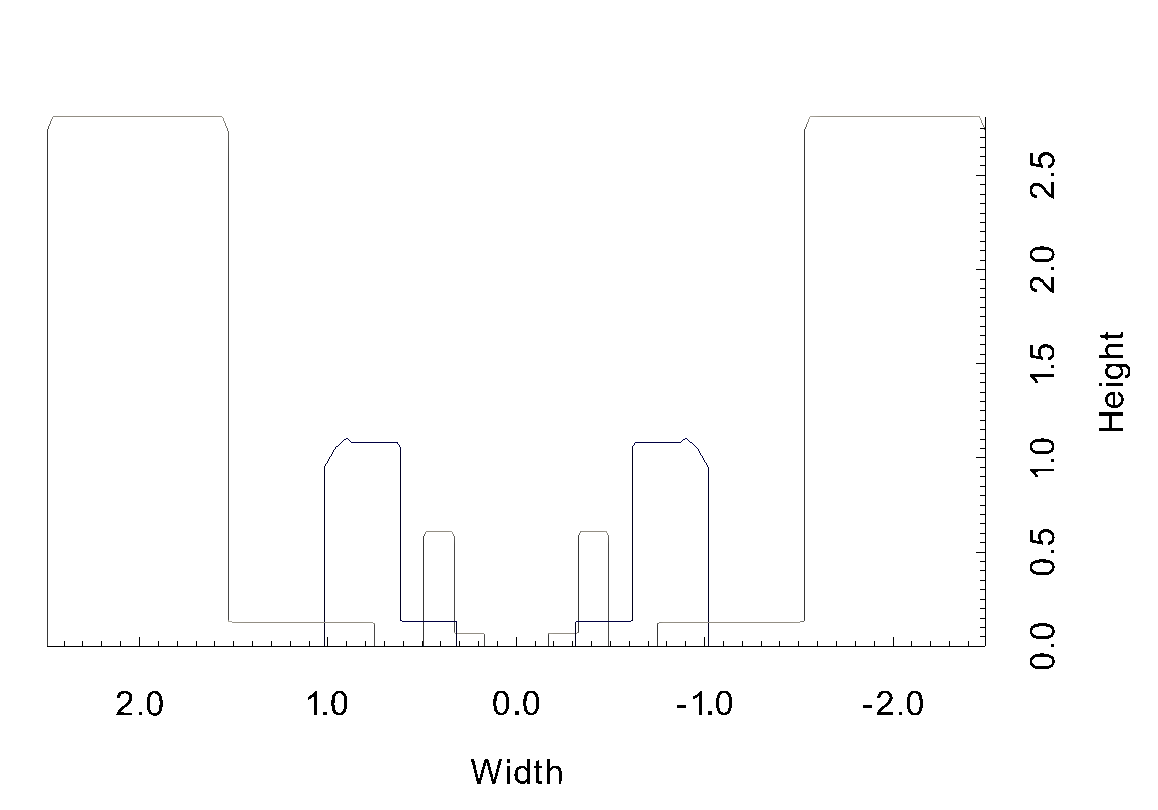
\includegraphics[width = 12 cm]{figs/vane_scaling}
    \caption{An image showing the three different vane configurations. The three-meter vanes (mid-sized set) 
      have a slight plotting artifact at the top outer corner, but this does not exist in the simulations. }
    \label{vane_scaling}
  \end{center}
\end{figure}


This document details investigations into the variation of the Solar Vortex (SoV) physical size and energy as a function of diameter of the apparatus. We consider 
three fully developed, averaged runs for system configurations that are identical excepting having been scaled to larger sizes. We will use 
system apparatus that have diameters of one, three and five meters. The design is two tiers, with a longer curved vane on the bottom tier providing a 
smoother and slower variation in angle as a function of radius. Each configuration has an outer angle of $0\degree$, and varying along a smooth curve 
depending on the square root of the radius inward to a maximum angle of $75\degree$. The ``baseline'' configuration was the three meter design, 
which was optimized over the coarse of a parameter sweep across inner and outer radius, heights, angles, etc. These different run 
definitions are completely defined in Table \ref{fig:scaling_table}. The results shown here are all temporally averaged, and are not sensitive to changes in the domain size.

%
% image of vane angle?
%
Figure \ref{vane_scaling} plots a vertical slice through the three vane sizes, to give the reader a sense of the 
scale between each configuration.

\begin{figure}[!htb]
\minipage{0.32\textwidth}
  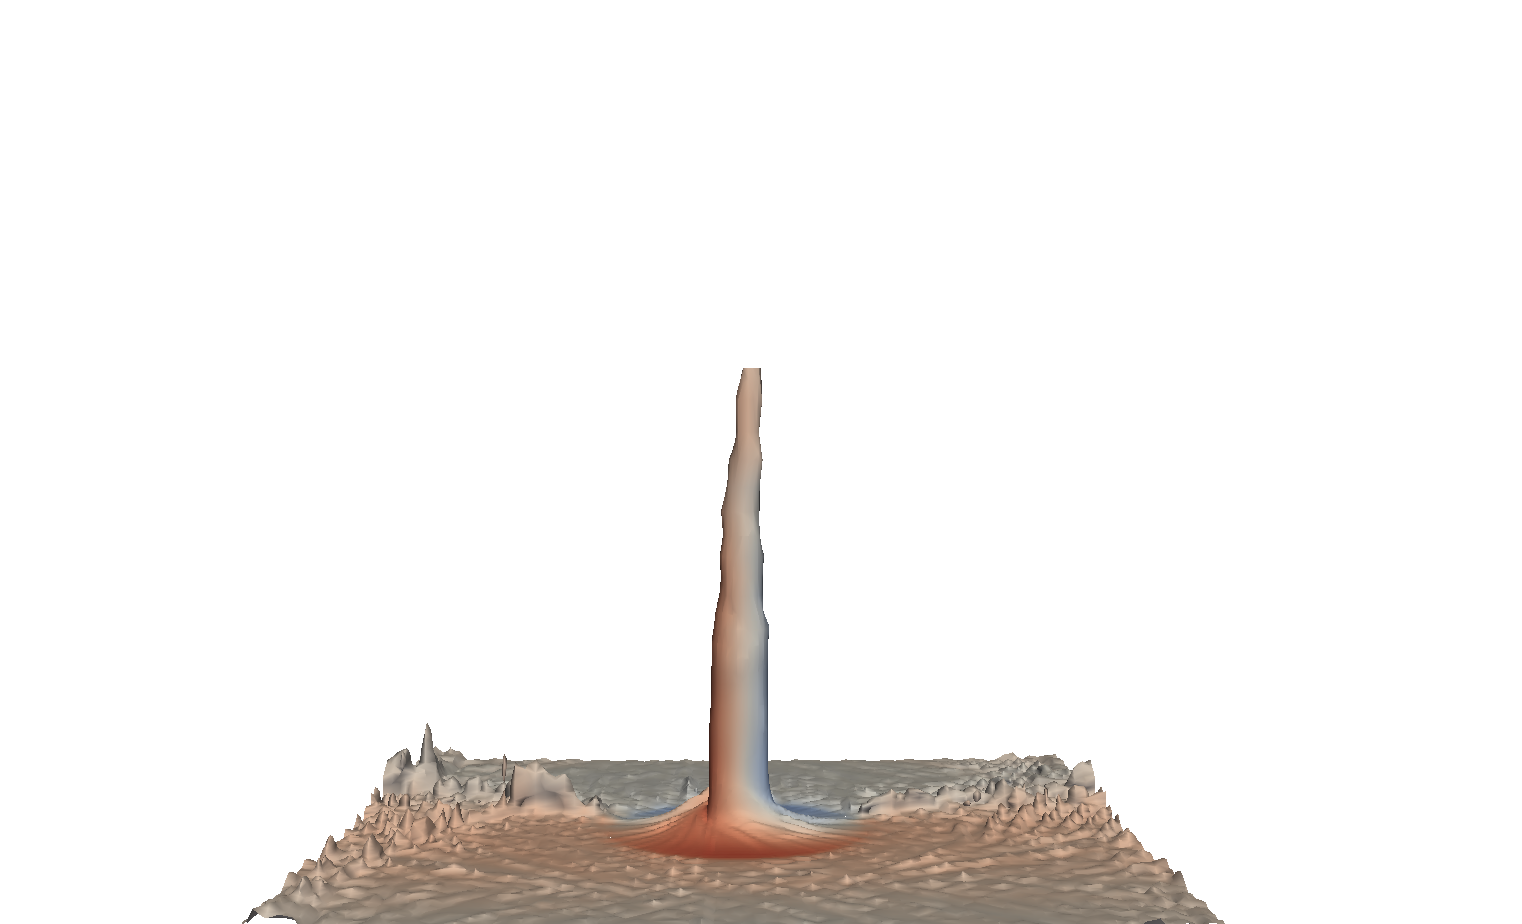
\includegraphics[width=\linewidth]{figs/1m_temp_iso}
  \caption{1m Apparatus}\label{fig:1m_scaling}
\endminipage\hfill
\minipage{0.32\textwidth}
  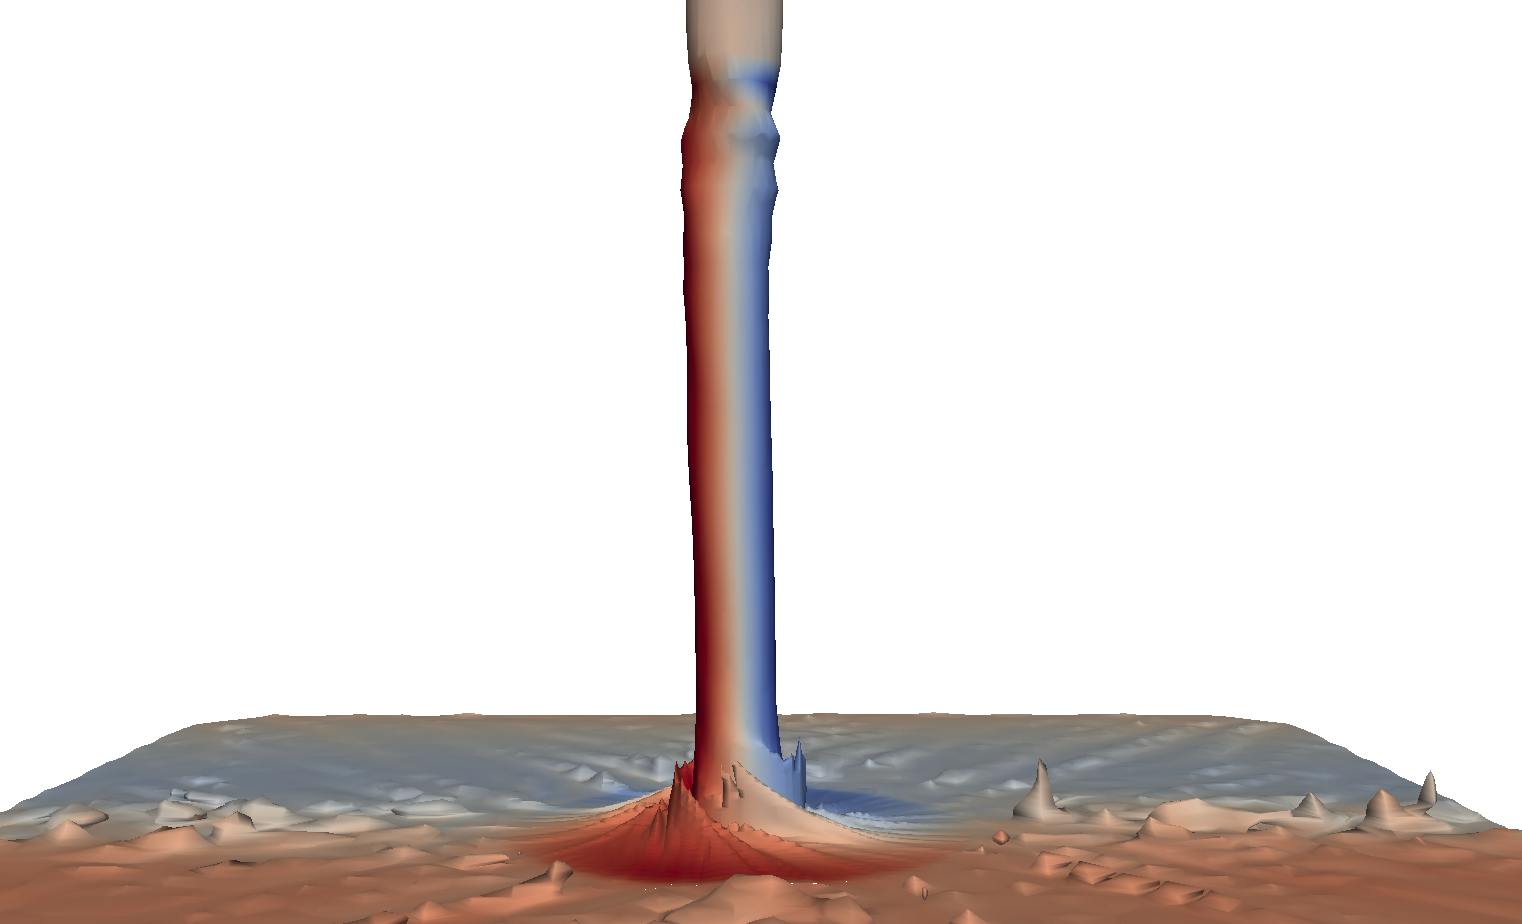
\includegraphics[width=\linewidth]{figs/3m_temp_iso}
  \caption{3m Apparatus}\label{fig:3m_scaling}
\endminipage\hfill
\minipage{0.32\textwidth}%
  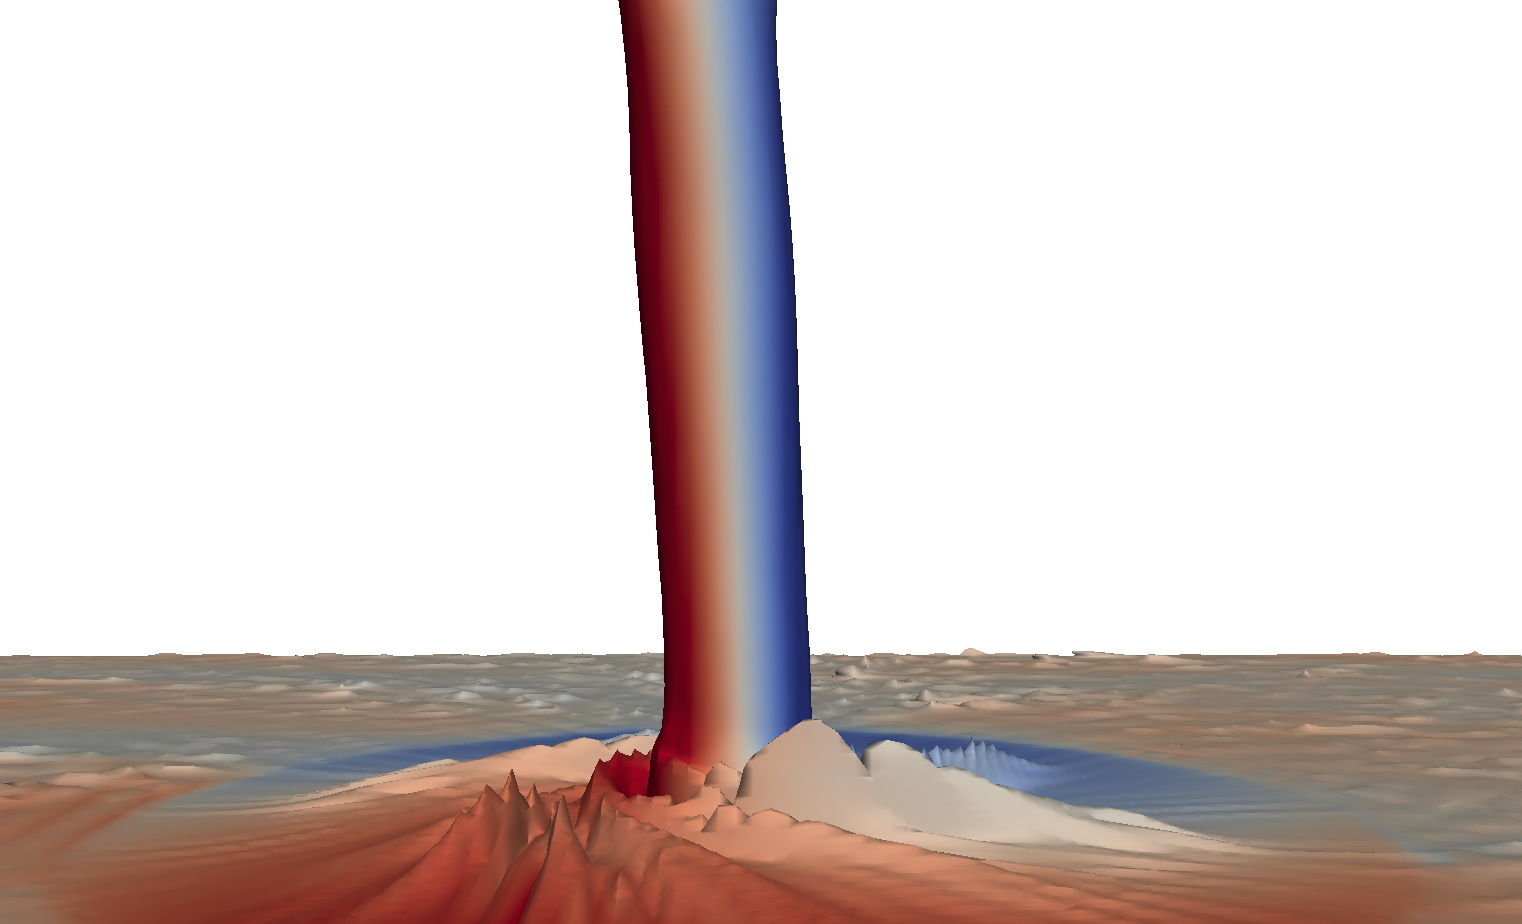
\includegraphics[width=\linewidth]{figs/5m_temp_iso}
  \caption{5m Apparatus}\label{fig:5m_scaling}
\endminipage
\end{figure}


\begin{figure}[!htb]
  \begin{center}
    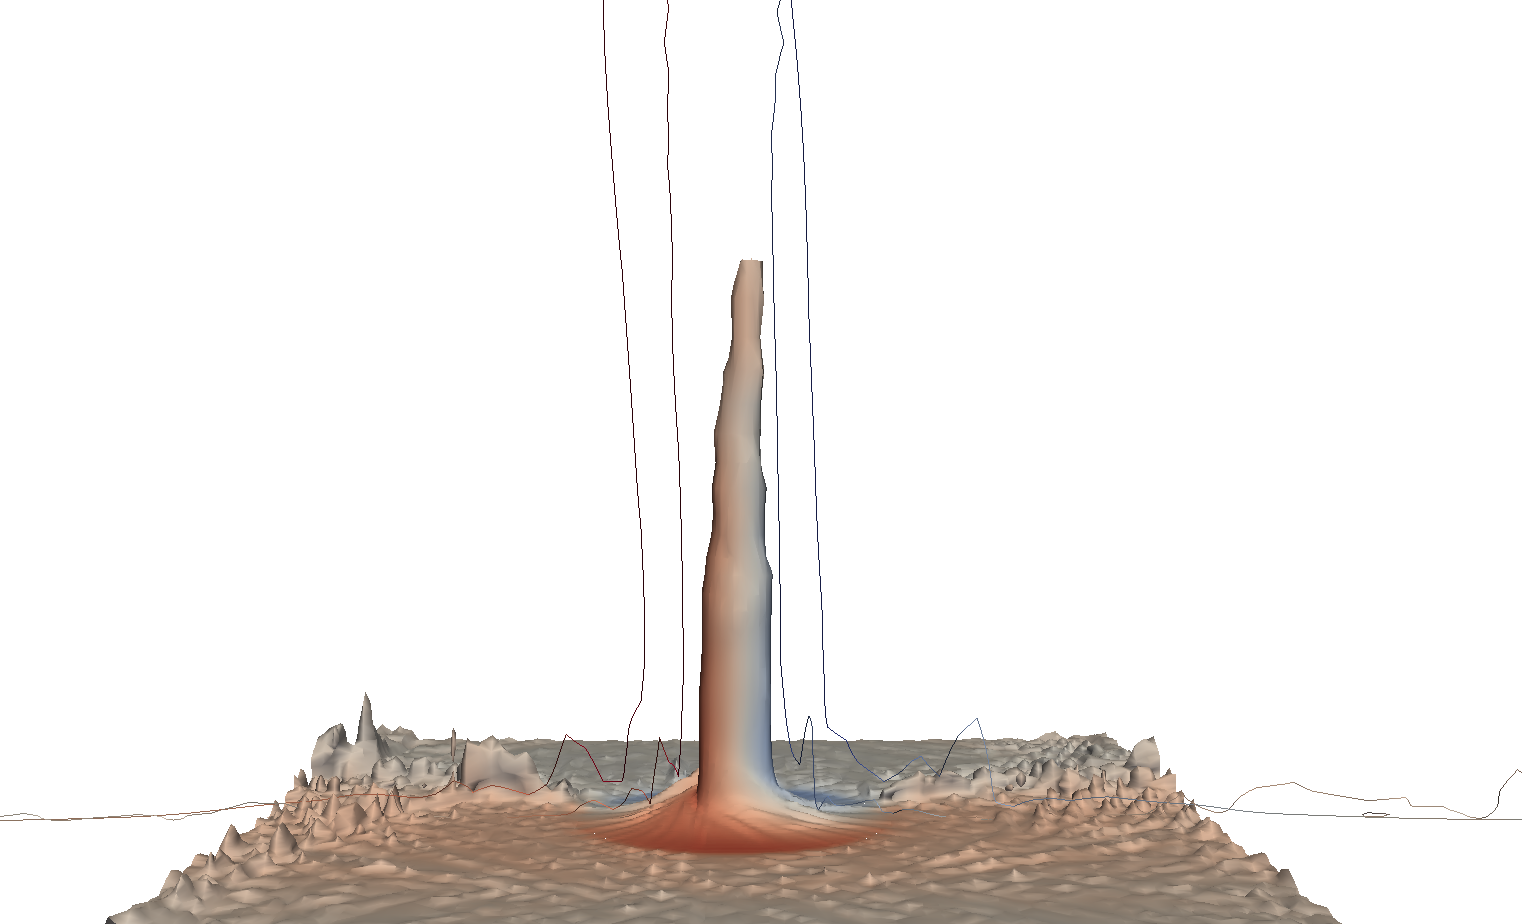
\includegraphics[width = 12 cm]{figs/temp_iso}
    \caption{Thermal Isocontours from the three different cases superimposed 
      on top of each other to show the growing extend of the thermal column at larger vane sizes. }
    \label{fig:scaling_slice}
  \end{center}
\end{figure}


An isocontour of the temperature field (contoured at 317 Kelvin) are shown in figures \ref{fig:1m_scaling}-\ref{fig:5m_scaling}. 
It is clear that as the vanes grow in size, the physical size of the thermal plume also increases. This is shown slightly more clearly in
 Figure \ref{fig:scaling_slice}. 

%
% probably need to plot the increase in diameter as a function of diameter 
%


\begin{figure}[!htb]
\minipage{0.32\textwidth}
  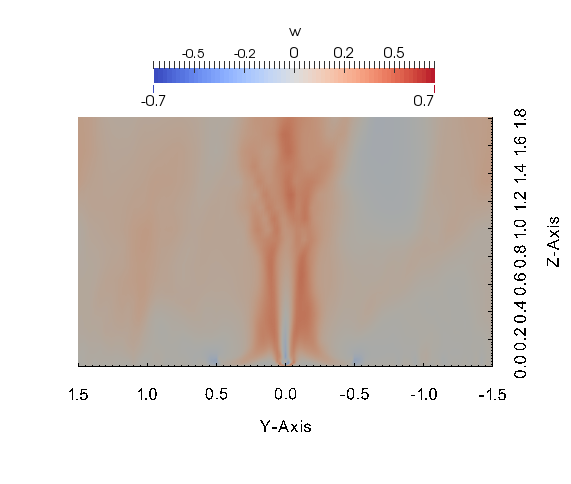
\includegraphics[width=\linewidth]{figs/w_scaled_1m}
  \caption{Vertical Velocity: 1m Apparatus}\label{fig:1m_vz}
\endminipage\hfill
\minipage{0.32\textwidth}
  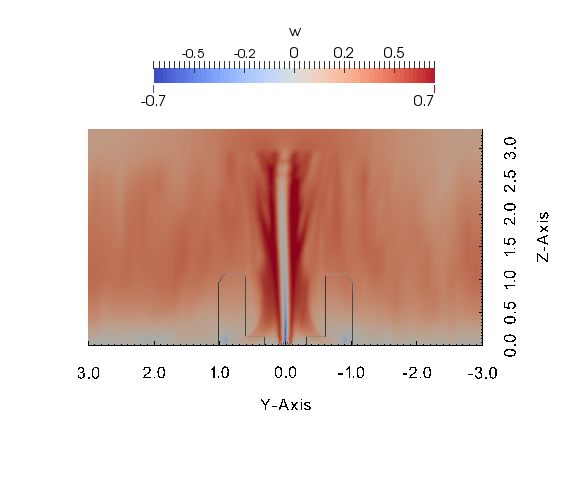
\includegraphics[width=\linewidth]{figs/w_scaled_3m}
  \caption{Vertical Velocity: 3m Apparatus}\label{fig:3m_vz}
\endminipage\hfill
\minipage{0.32\textwidth}%
  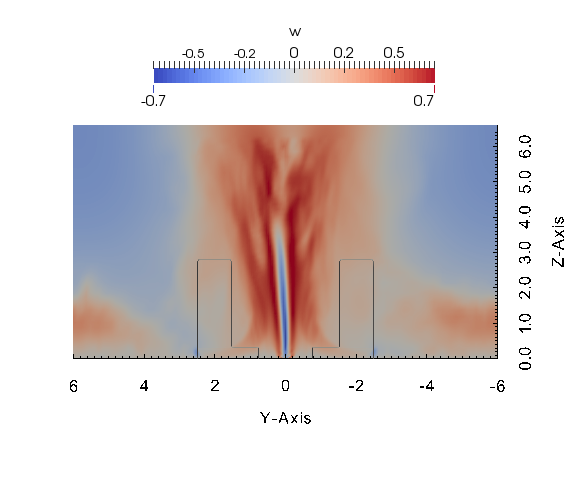
\includegraphics[width=\linewidth]{figs/w_scaled_5m}
  \caption{Vertical Velocity: 5m Apparatus}\label{fig:5m_vz}
\endminipage
\end{figure}
 
Figure \ref{fig:scaling_slice} shows the vertical velocity for each of the three cases. It is more clear here than in the thermal column case
that there exists a qualitatively similar structure between each of the three cases. 


%
% just a figure
%

  %% \begin{figure}[!htb]
  %%   \begin{center}
  %%    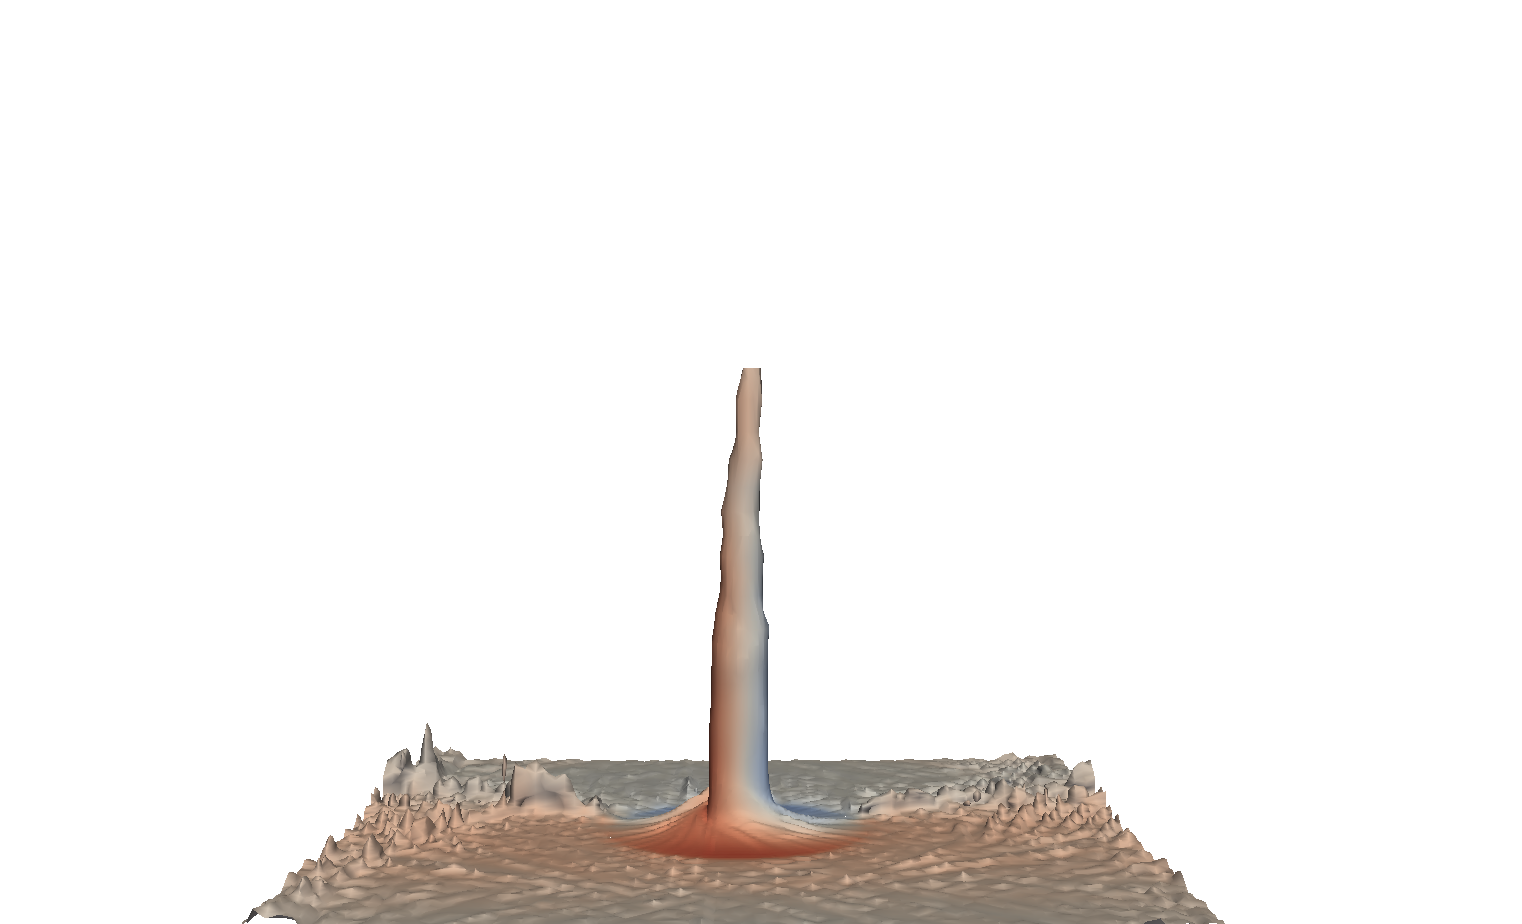
\includegraphics[width = 12 cm]{figs/1m_temp_iso}
  %%    \caption{1m }
  %%    \label{lab}
  %%   \end{center}
  %% \end{figure}


\end{document}
